\documentclass[border=5pt]{standalone}
\usepackage{tikz}
\usepackage{amsmath}
\begin{document}
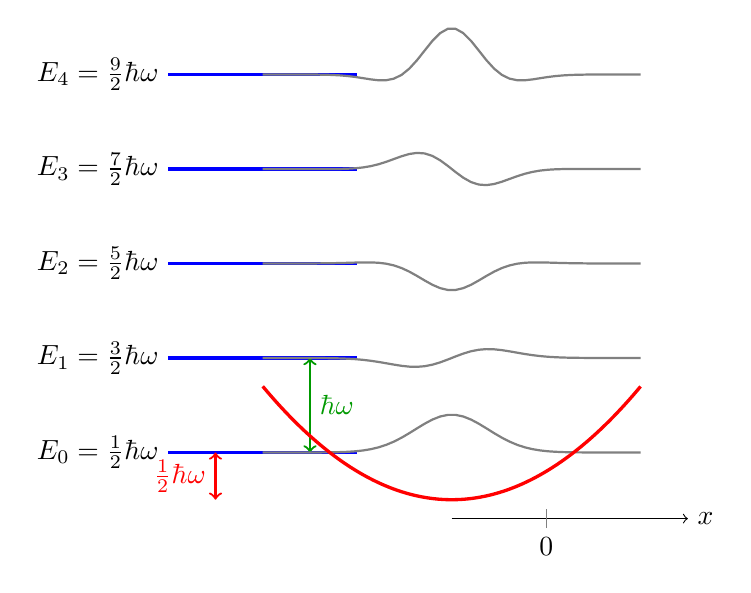
\begin{tikzpicture}[scale=1.2]
    % 能级
    \foreach \n/\y/\label in {0/0.5/{E_0=\frac{1}{2}\hbar\omega},1/1.5/{E_1=\frac{3}{2}\hbar\omega},2/2.5/{E_2=\frac{5}{2}\hbar\omega},3/3.5/{E_3=\frac{7}{2}\hbar\omega},4/4.5/{E_4=\frac{9}{2}\hbar\omega}} {
        \draw[very thick,blue] (-1,\y) -- (1,\y);
        \node[left] at (-1,\y) {$\label$};
    }
    
    % 零点能标注
    \draw[<->,thick,red] (-0.5,0) -- (-0.5,0.5);
    \node[left,red] at (-0.5,0.25) {$\frac{1}{2}\hbar\omega$};
    
    % 能级间距标注
    \draw[<->,thick,green!60!black] (0.5,0.5) -- (0.5,1.5);
    \node[right,green!60!black] at (0.5,1) {$\hbar\omega$};
    
    % 波函数示意 (右侧)
    \draw[thick,gray,domain=-2:2,samples=50] plot ({2+\x},{0.5 + 0.4*exp(-\x*\x/0.3)});
    \draw[thick,gray,domain=-2:2,samples=50] plot ({2+\x},{1.5 + 0.4*\x*exp(-\x*\x/0.3)});
    \draw[thick,gray,domain=-2:2,samples=50] plot ({2+\x},{2.5 + 0.4*(4*\x*\x-2)*exp(-\x*\x/0.3)/2.83});
    \draw[thick,gray,domain=-2:2,samples=50] plot ({2+\x},{3.5 + 0.4*(8*\x*\x*\x-12*\x)*exp(-\x*\x/0.3)/6});
    \draw[thick,gray,domain=-2:2,samples=50] plot ({2+\x},{4.5 + 0.4*(16*\x*\x*\x*\x-48*\x*\x+12)*exp(-\x*\x/0.3)/9.8});
    
    % x轴
    \draw[->] (2,-0.2) -- (4.5,-0.2) node[right]{$x$};
    \draw[gray] (3,-0.3) -- (3,-0.1);
    \node[below] at (3,-0.3) {$0$};
    
    % 势能曲线
    \draw[very thick,red,domain=-2:2,samples=100] plot ({2+\x},{0.3*\x*\x});
\end{tikzpicture}
\end{document}
